% !TeX encoding = UTF-8
% !TeX spellcheck = en_US
\section{Implementation}
\IEEEPARstart{T}his chapter will clarify the development history, 
discovered bugs and design decisions taken.
Let us first take a look on programs 
which already existed when this project started and 
why they have or have not been used  for KeFaX 
and then go into the implementation details.

\subsection{Using existing compilers / compiler-generators}
C/C++ are very complex programming languages with a lot of disambiguties,
lots of different revisions (e.g. ANSI C, ISO/IEC C99\cite{ISOC99}, C++11) and a 
huge amount of compiler specific extensions
(GNU GCC extensions, etc.). 
The Linux kernel makes use of some of the GNU C extensions.
Therefore, it is not possible to compile the vanilla sources of the Linux kernel with Clang
LLVM yet - the Clang front-end\cite{ClangIntro} would provide a nice abstract syntax tree (AST), 
e.g., as a XML file.
Clang claims to be fully GNU gcc compliant and is
used as a replacement of the GNU compiler suite already in
several projects because of its advanced static code analyzing
capabilities. Part of the function declaration of the main-
function for the hello-world example can be found in code
listing \ref{clangast}.
\lstinputlisting[language=XML, firstline=1, lastline=10,
frame=single,extendedchars=true,label=clangast,caption={part of the clang-ast output file},
breaklines=true,]{code/clang-ast.txt}
Another issue is still that their is only limited support for 
traversing, working and exporting the AST for further investigations
by other applications.

GNU gcc itself provides its internal data structures to external programs.
Applications might use this information and provide AST as XML, e.g.
XOgastan\cite{XOgastan} or 
GCC\_XML \cite{gccxml}.
An example
output for gcc-xml can be seen in source code listing \ref{gccxml}
\lstinputlisting[frame=single,extendedchars=true,label=gccxml,language=XML,
  caption={part of the gccxmloutput.xml file},
  firstline=517, lastline=523,
  breaklines=true,]{code/gccxmloutput.xml}
When at first this method seemed promising, it turned out
that gcc-xml is generating too much non-descriptive IDs, is
sometimes buggy and that the GNU gcc itself is not producing
an easily iterate-able AST itself.
\\ \ \\
Compiler compilers are based on processing formal
grammars. The research in theoretic computer science has led
to the automation of generating scanners and parsers out of an
existing formal description text of the programming language
(wherefore often the EBNF - extended Backus-Naur-Form - is
used as a notation).
For compiler generators like Coco/R\cite{COCOR}
(which has been developed at the SSW
institute at the JKU in Linz), 
GNU's implementation of Yacc called Bison\cite{Bison}, etc. there is no unique 
and/or clear EBNF available for C/C++ which would also include most of the GNU C extensions.
One disadvantage of compiler
compilers is the mixture of multiple languages (one language
for describing the scanning/parsing process mixed with the
source code statements for the resulting compiler). Another
disadvantage is that often C/C++ EBNF descriptions lack
language features like the GNU C extensions or others. But the worst
matter is that all information about preprocessor statements
in C and C++ are lost because EBNFs can not deal with
include or define macros.
EBNF profiles of various programming languages can
be found in the grammarware Github repository\cite{Grammarzoo}.
A little out-dated grammar description 
for GNU GCC can be found at \cite{GNUCEBNF}.
\\ \ \\
The problem with most of the evaluated tools is that they are either 
not available anymore or are out-dated or buggy.
But even if they would work, 
the next question is how to build-up the AST, 
which tools and which data structures to use and 
how much effort would be required to do so \dots

\subsection{Reverse Engineering}
How about using {\it EMF (Eclipse Modeling Framework)}
\cite{Eclipse_EMF}
\cite{steinberg2008emf}
instead? EMF provides rich APIs for processing and transforming 
a model into other models or code.
An tutorial on EMF can, for example, be found at 
\cite{EMF_Tutorial}.
So which projects
exist for working with C/C++ in conjunction with EMF?

\subsubsection{EMF4CPP}
The first hit on Google when searching for EMF and C/C++ is 
{\it EMF4CPP}
\cite{EMF4CPP} 
\cite{senac2010emf4cpp}. 
It provides the ability to work with EMF models inside a 
C++ project
(just like Java is supported out-of-the-box) by including the 
library which is part of EMF4CPP.
Another feature of this open-source project is to enable the 
generation of C++ source text out of an Ecore model.
It also comes with a XText artifact for importing C++ code 
into an EMF model.
Unfortunately, as the goal of EMF4CPP is a different one,
it only supports a small subset of C++, 
e.g. it is not possible to 
use macro directives, embedded C or assembler code.
EMF4CPP is, therefore, more similar to the 
{\it Javascript for EMF (JS4EMF)} project
\cite{JavaScript4EMF_1}
\cite{JavaScript4EMF_2}.
It is not possible 
to parse the Linux kernel with
this project.

\subsubsection{Eclipse MoDisco}
So far, the approaches have been disappointing because
every one had major disadvantages. But the method described
in this section about Eclipse MoDisco seemed promising.

The paper  "Model-Based Mining of Source Code Repositories"
\cite{scheidgen2014model}
written by
Markus Scheidgen and Joachim
Fischer describes how they utilized {\it Eclipse MoDisco}
for reverse-engineering of open source code repositories
like GitHub to gain static code analysis metrics about
Java applications. 

{\it Eclipse MoDisco} 
\cite{Modisco_1}
\cite{bruneliere2010modisco}
\cite{bruneliere2014modisco}.
claims to provide "an
extensible framework to develop model-driven tools to support
use-cases of existing software modernization". 

\begin{figure}[ht]
    \centering
	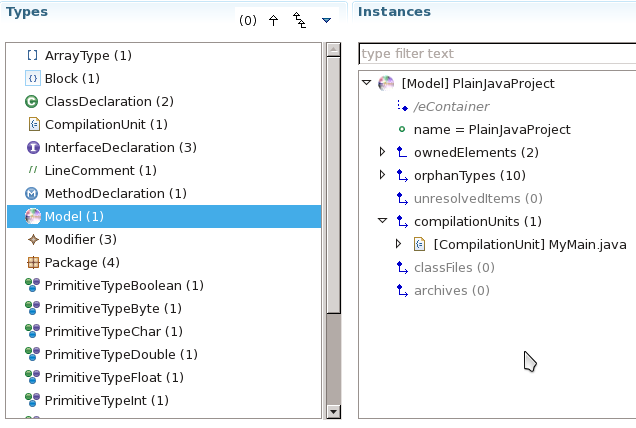
\includegraphics[scale=0.5]{images/JavaAST-2}
	\caption{Eclipse MoDisco model for a simple Java project}
    \label{fig:JavaAST2}
\end{figure}

\begin{figure}[ht]
    \centering
	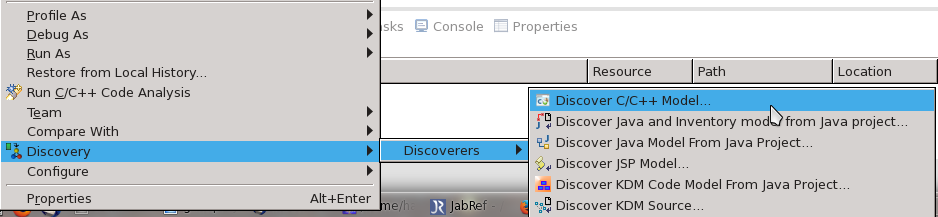
\includegraphics[scale=0.35]{images/discoverer}
	\caption{Using Eclipse MoDisco}
    \label{fig:discoverer}
\end{figure}
\FloatBarrier

It is a reverse-engineering framework which is built on top of the
{\it Eclipse EMF} (Eclipse Modeling Framework).
This would solve the question of which data structure / abstract syntax tree
to use for storage.
Discoverers are a set of Eclipse plug-ins that provide an importer/parser for a 
certain programming language.
There exist discoverers for Java, JSP, JSON and many more.
Unfortunately, {\it Eclipse MoDisco discoverers} for C and C++ 
did not exist when starting this project.
In the Eclipse forum in a thread called ``Looking for c/c++ discoverer''
\cite{C_Discoverer} it was suggested to piggy-back use 
{\it Eclipse CDT ((Compiler development tools))}
\cite{Eclipse_CDT}\cite{piatov2012using} to implement a C/C++ discoverer.

{\it Eclipse CDT} supports C/C++ and can deal with most of the GNU C extensions
and pre-processing directives but it has 
a deeply nested code structure that is not always easy to deal with when 
walking the tree, as it can be seen in code snippet \ref{IASTNode}.

\lstinputlisting[language=Java, firstline=1, lastline=39,frame=single,label=IASTNode,
caption={Javadoc subinterfaces of  IASTNode},
breaklines=true,]{code/iastnode.txt}

Therefore, it was decided to change from {\it Eclipse CDT} to a different parsing 
technology. 

\subsubsection{ANTLR, EMFText and Xtext}
Luckily there is an {\it ANTLR} grammar available 
at the {\it antlr/grammars-v4} Github repository \cite{C_v4}.
which already includes
most of the GNU C extensions. 
"ANTLR (ANother Tool for Language Recognition)
is a powerful parser generator for reading, processing, executing, 
or translating structured text or binary files.
 It's widely used to build languages, tools, and frameworks. 
 From a grammar, 
 ANTLR generates a parser that can build and walk parse trees."\cite{Antlr}
There exist bindings for different programming languages including Java
(in which most of its parts are also developed) but {\it ANTLR} does not
support exporting to {\it Eclipse EMF}.

{\it ANTLR} itself is used by two Text-To-Model tools for the 
{\it Eclipse IDE}:
{\it EMFText} and {\it XText}. 
Both provide the possibility to engineer DSLs and use the automated 
generation of advanced text editors which support syntax highlighting,
error recovering and auto-completion. 
{\it XText} has the advantage compared to {\it EMFText} that it is
an official Eclipse project and that it can automatically generate
an Ecore meta-model out of a grammar description file. 
Both use a version three of {\it ANTLR}
\cite{ANTLR4_XText}
\cite{ANTLR4_EMFText}
which has some disadvantages
compared to the newer re-written {\it ANTLR v4} which supports
some automatically left-recursion resolution and, therefore,
does not need semantic predicates anymore.
Even if almost all complex EBNF grammars 
use left-recursions,
most of them can be re-factored to avoid disambiguates.
\\ \ \\
But there are cases in the C programming languages
which require semantic predicates
(e.g., to distinguish between declarations
and function definitions) to remove left-recursion from the grammar. 
For more information on semantic predicates see 
\cite{parr1994adding} and \cite{SemPreds}.
{\it ANTLR} in version four does not need semantic predicates anymore
for parsing C/C++,
version three supports them at least.
Unfortunately, even if {\it EMFText} and {\it XText} both use {\it ANTLR} in version three,
they do not support semantic predicates (they only support syntactical predicates).

{\it XText} internally generates an ANTLR grammar file (e.g., {\it InternalParser.g})
out of the DSL grammar description file (e.g., {\it Parser.xtext}).
When semantic predicates where inserted into this intermediate file and this
grammar was then fed into the {\it ANTLR} application as an input, it was possible
to create a valid C parser. 
Therefore, it was necessary to add semantic predicate support to {\it XText} first,
to avoid patching of the intermediate file all the time.
This has been implemented in \url{https://github.com/timeraider4u/xtext}
\cite{Xtext_mod}
which is a fork of the official {\it Xtext} source code.
When this was done, the need for an own C pre-processor has arisen
which should be able to also gain information on which conditionals 
where taken, to resolve pre-processor macros and so on\dots
The C pre-processor and parser
have then been tested against various test code and 
parts of the libc implementation.
Afterwards the C pre-processor and parser 
combination have been integrated into an {\it Eclipse MoDisco} discoverer
and the final result
has been tested against the Linux kernel. 
Whenever
an error occurred 
new JUnit test cases have been added and the grammar files
have been extended to support these language features as well.
Not all GNU C extensions are supported yet (they are far too many).
\\ \ \\
Unfortunately, some issues still remain unsolved at this moment, 
including some cases that can lead to {\it OutOfMemory exceptions}.
Even moving from the default {\it EMF XMI storage back-end} to
{\it NeoEMF} could not resolve this problem satisfactorily.
{\it NeoEMF}\cite{NeoEMF}
(previously called {\it Neo4EMF}) \cite{benelallam2014neo4emf}
is a storage back-end for {\it EMF} models. 
It provides adapters for {\it MapDB} and the graph database
{\it Neo4J} to store/deal with {\it EMF} models.

Some analysis with the Eclipse Memory Analyzer (MAT)
\cite{Eclipse_MAT}
\cite{Eclipse_MAT_2}
has shown that there seem to be two reasons:
The first one is that XText uses its own lazy loading implementation
which conflicts with using a separate storage back-end
(e.g., see \cite{NeoEMF_Xtext}).
The second reason is that {\it Eclipse MoDisco} currently 
only supports {\it XMI} serialization out-of-the-box and,
therefore, the {\it EMF model browser} can not deal 
with the lazy loading algorithm
(which is used by {\it NeoEMF})
correctly.

\subsection{MORE TO DO}
More detailed descriptions coming soon\dots

%'[antlr-interest] Solution for specialStateTransition exceeding 65k' - MARC
% http://marc.info/?l=antlr-interest&m=127495195324148
%
% Eclipse Community Forums: TMF (Xtext) » [Xtext] Embedding ANTLR code into XText?
% https://www.eclipse.org/forums/index.php?t=msg&th=1069632
%
% Bug 362901 – Add @Nullable, @NonNull support
% https://bugs.eclipse.org/bugs/show_bug.cgi?id=362901
% and
% Bug 428088 – @since tags should be generated to both getters and setters
% https://bugs.eclipse.org/bugs/show_bug.cgi?id=428088
%
% Bug 475615 – Support "git clone --depth" in CloneCommand
% https://bugs.eclipse.org/bugs/show_bug.cgi?id=475615
%
% Open Source Software Metrics by Resource Standard 
% Software Source Code Metrics For C, C++ and Java
% http://msquaredtechnologies.com/m2rsm/rsm_software_project_metrics.htm
